\chapter{Entwurf}
Um das benötigte Plug-in System zu realisieren, boten sich verschiedene
\first{Application Frameworks} an, die eine entsprechende Funktionalität
bereitstellen und somit als Programmbasis für die  Pipeline dienen konnten.
\index{Application Framework}
Die Wahl fiel hier auf das \first{OSGi Framework} \first{Equinox}, welches von
der \name{Eclipse Fundation} entwickelt wird und auch die Basis für die
Entwickungsumgebung \name{Eclipse} darstellt.
\index{Equinox}
\index{OSGi}
\index{OSGi Framework|see{OSGi}} 
\index{Eclipse}

\name{Eclipse Equinox} ist in Java geschrieben, was der Portierbarkeit der
Pipeline entgegenkommt. Ausserdem bietet die Framework-Architektur maximale
Modularisierung, wodurch sich Anwendungen auf \name{Equinox}-Basis durch
hervorragende Erweiterbarkeit und Skalierbarkeit auszeichnen.
\section{Das OSGi Framework}

%\begin{wrapfigure}{r}{9.0cm}
%	\begin{center}
%		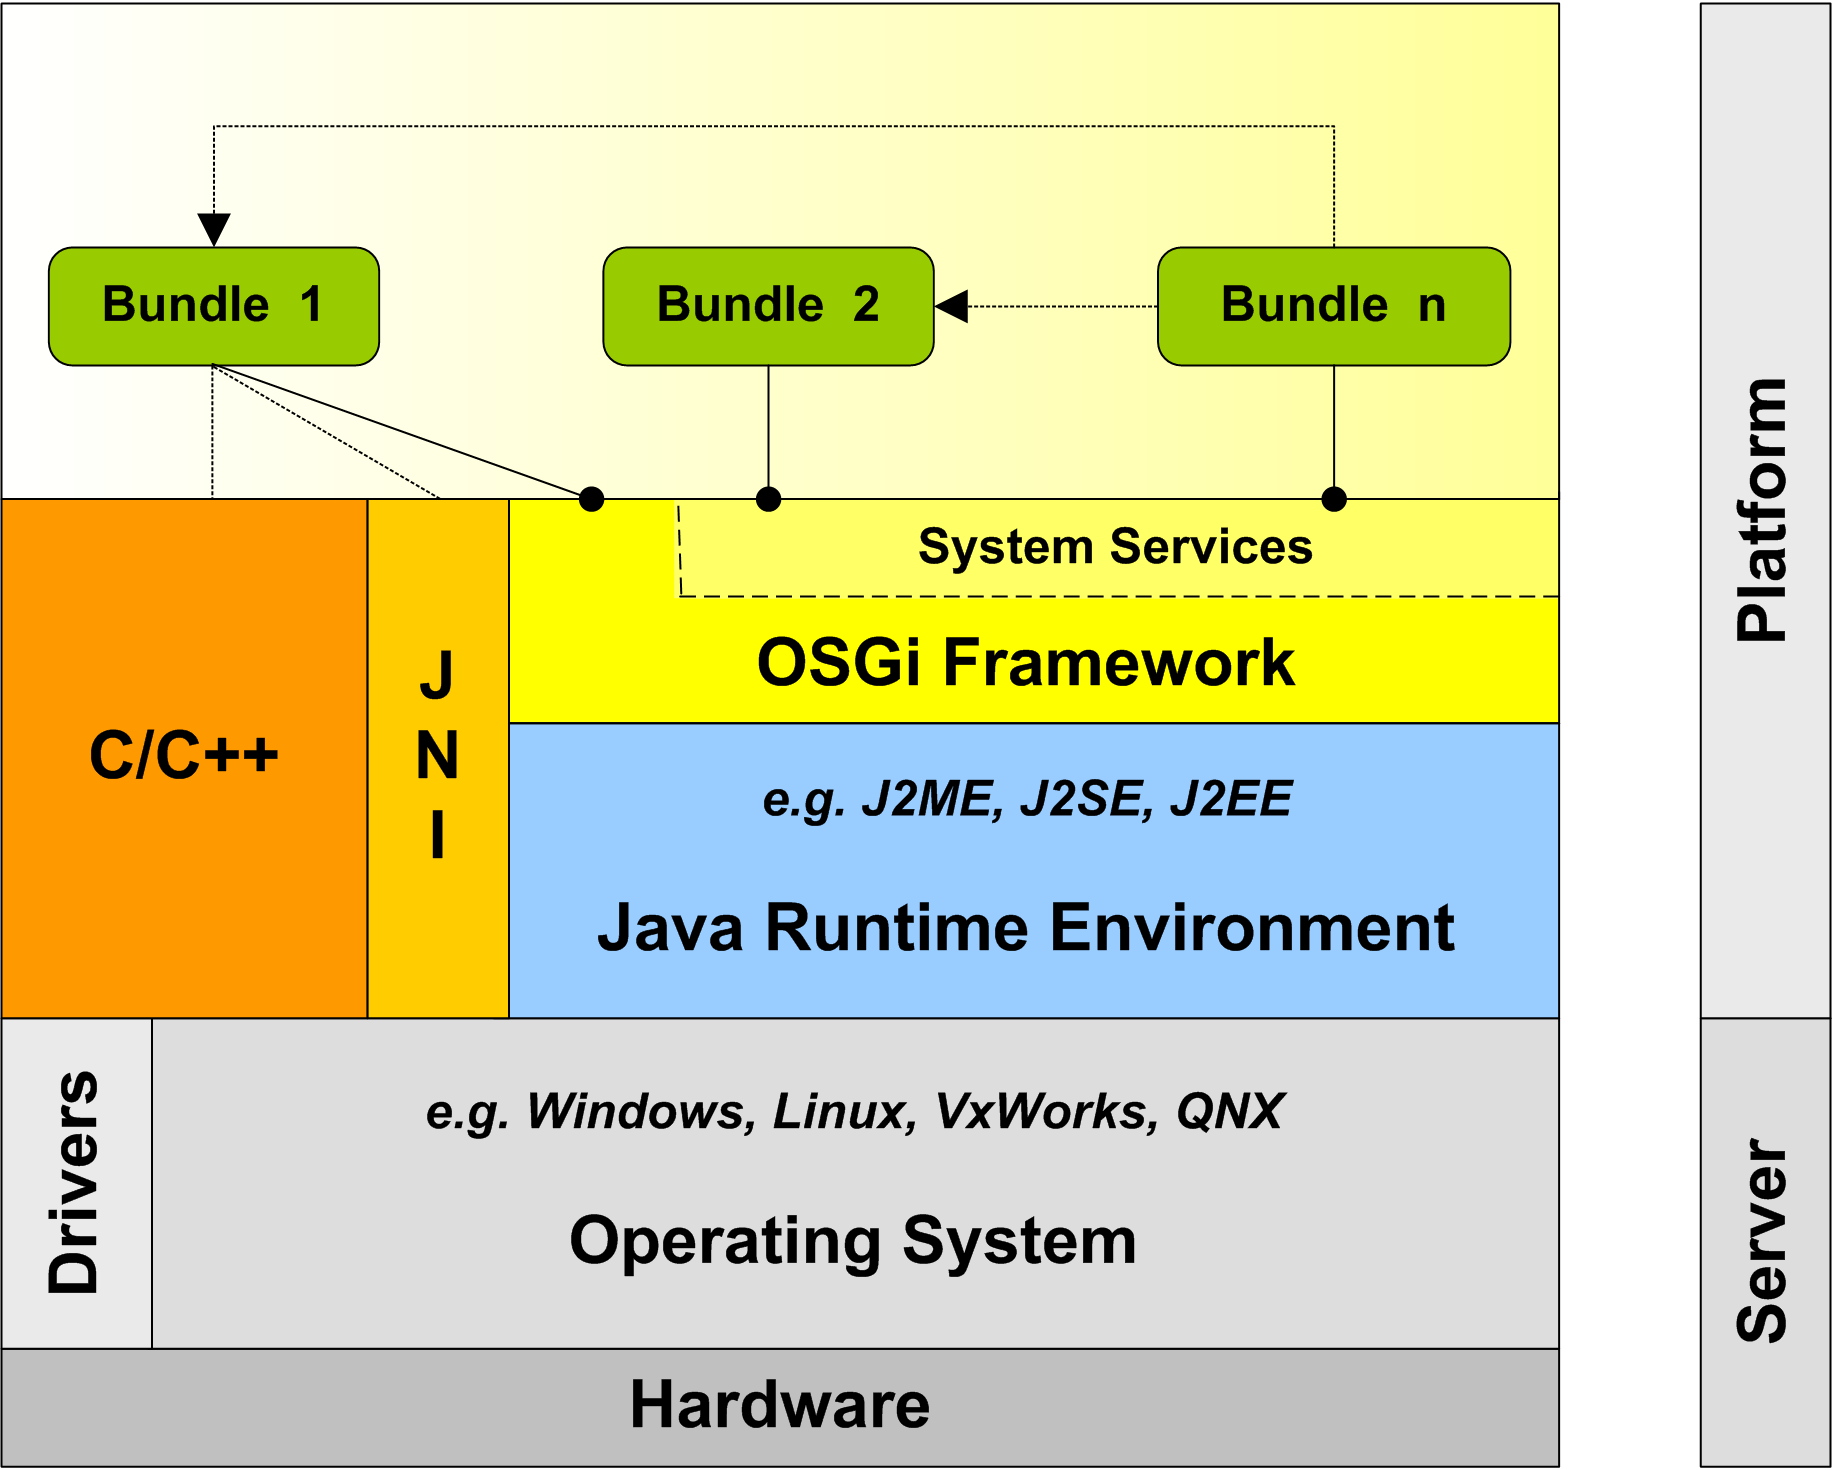
\includegraphics[width=8.5cm]{pics/osgi_layer.png}
%	\caption{something, citing}
%	\end{center}
%	\label{fig:hmm}
%\end{wrapfigure}

Die \name{OSGi Alliance}, früher \enquote{\textit{Open Services Gateway
initiative}}, ist ein Zusammenschluß verschiedener Unternehmen, wie z.B. IBM,
Oracle oder Sun Microsystems.
\index{OSGi Alliance}
\index{OSGi|see{OSGi Alliance}}
\index{Open Services Gateway|see{OSGi Alliance}}
Sie spezifiziert die \first{OSGi Service Platform}, eine Java-basierte
Softwareplattform, die dem Pattern des \first{Komponentenmodell} folgt.
% footnote is von wikipedia !!!
\footnote{nach Gruhn und Thiel\citep{gruhn_komponentenmodelle_2000}:
\enquote{Ein Komponentenmodell legt einen Rahmen für die Entwicklung [..] von
Komponenten fest, der strukturelle Anforderungen hinsichtlich Verknüpfungs-
bzw. Kompositionsmöglichkeiten sowie verhaltensorientierte Anforderungen
hinsichtlich Kollaborationsmöglichkeiten an die Komponenten stellt.}}
Einzelne Komponenten, sogenannte \first{Bundles}, können der Anwendung
dynamisch hinzugefügt und wieder entfernt werden ohne dass ein erneutes
Kompilieren oder Starten der Anwendung nötig ist.
%%% hiernochmal %%% 
Abhängigkeiten zwischen Bundles werden dabei automatisch aufgelöst; ein
intelligentes Versionsmanagement steht ebenfalls zur Verfügung.
\index{OSGi Service Platform}
\index{Bundle}

Neben dem Komponentenmodell verwirklicht die Architektur des OSGi Frameworks
auch Elemente einer \first{Service Orientierten Architektur}.
\footnote{Unter \enquote{serviceorientierte Architektur} oder auch
\enquote{dienstorientierte Architektur} versteht man ein Softwaredesign, dass
sich durch sogenannte Dienste oder auch Services auszeichnet. Diese können
appliktaions-global an einer Registry angemeldet und abgefragt werden.
Sie stellen dabei eine Schnittstelle zu bestimmten Funktionen bereit, ohne
dabei die zu Grunde liegende Implementierung preiszugeben.}
So stellt das Framework eine globale Registry (\first{Service Registry})
bereit, an der Bundles \first{Dienste} bzw. \first{Services} anmelden und
abfragen können.
Ein \enquote{Dienst} ist hierbei eine Schnittstelle,
über die eine bestimmte Funktionalität anwendungsweit bereitgestellt wird.
\index{Dienst}
\index{Registry|see{Service Registry}}
\index{Service Registry}
\index{Service}
% OSGi Framework = OSGi Service Platform without OSGi Standard Services 13
\citep{wtherich_die_2008}

\begin{figure}[p]
	\begin{center}
		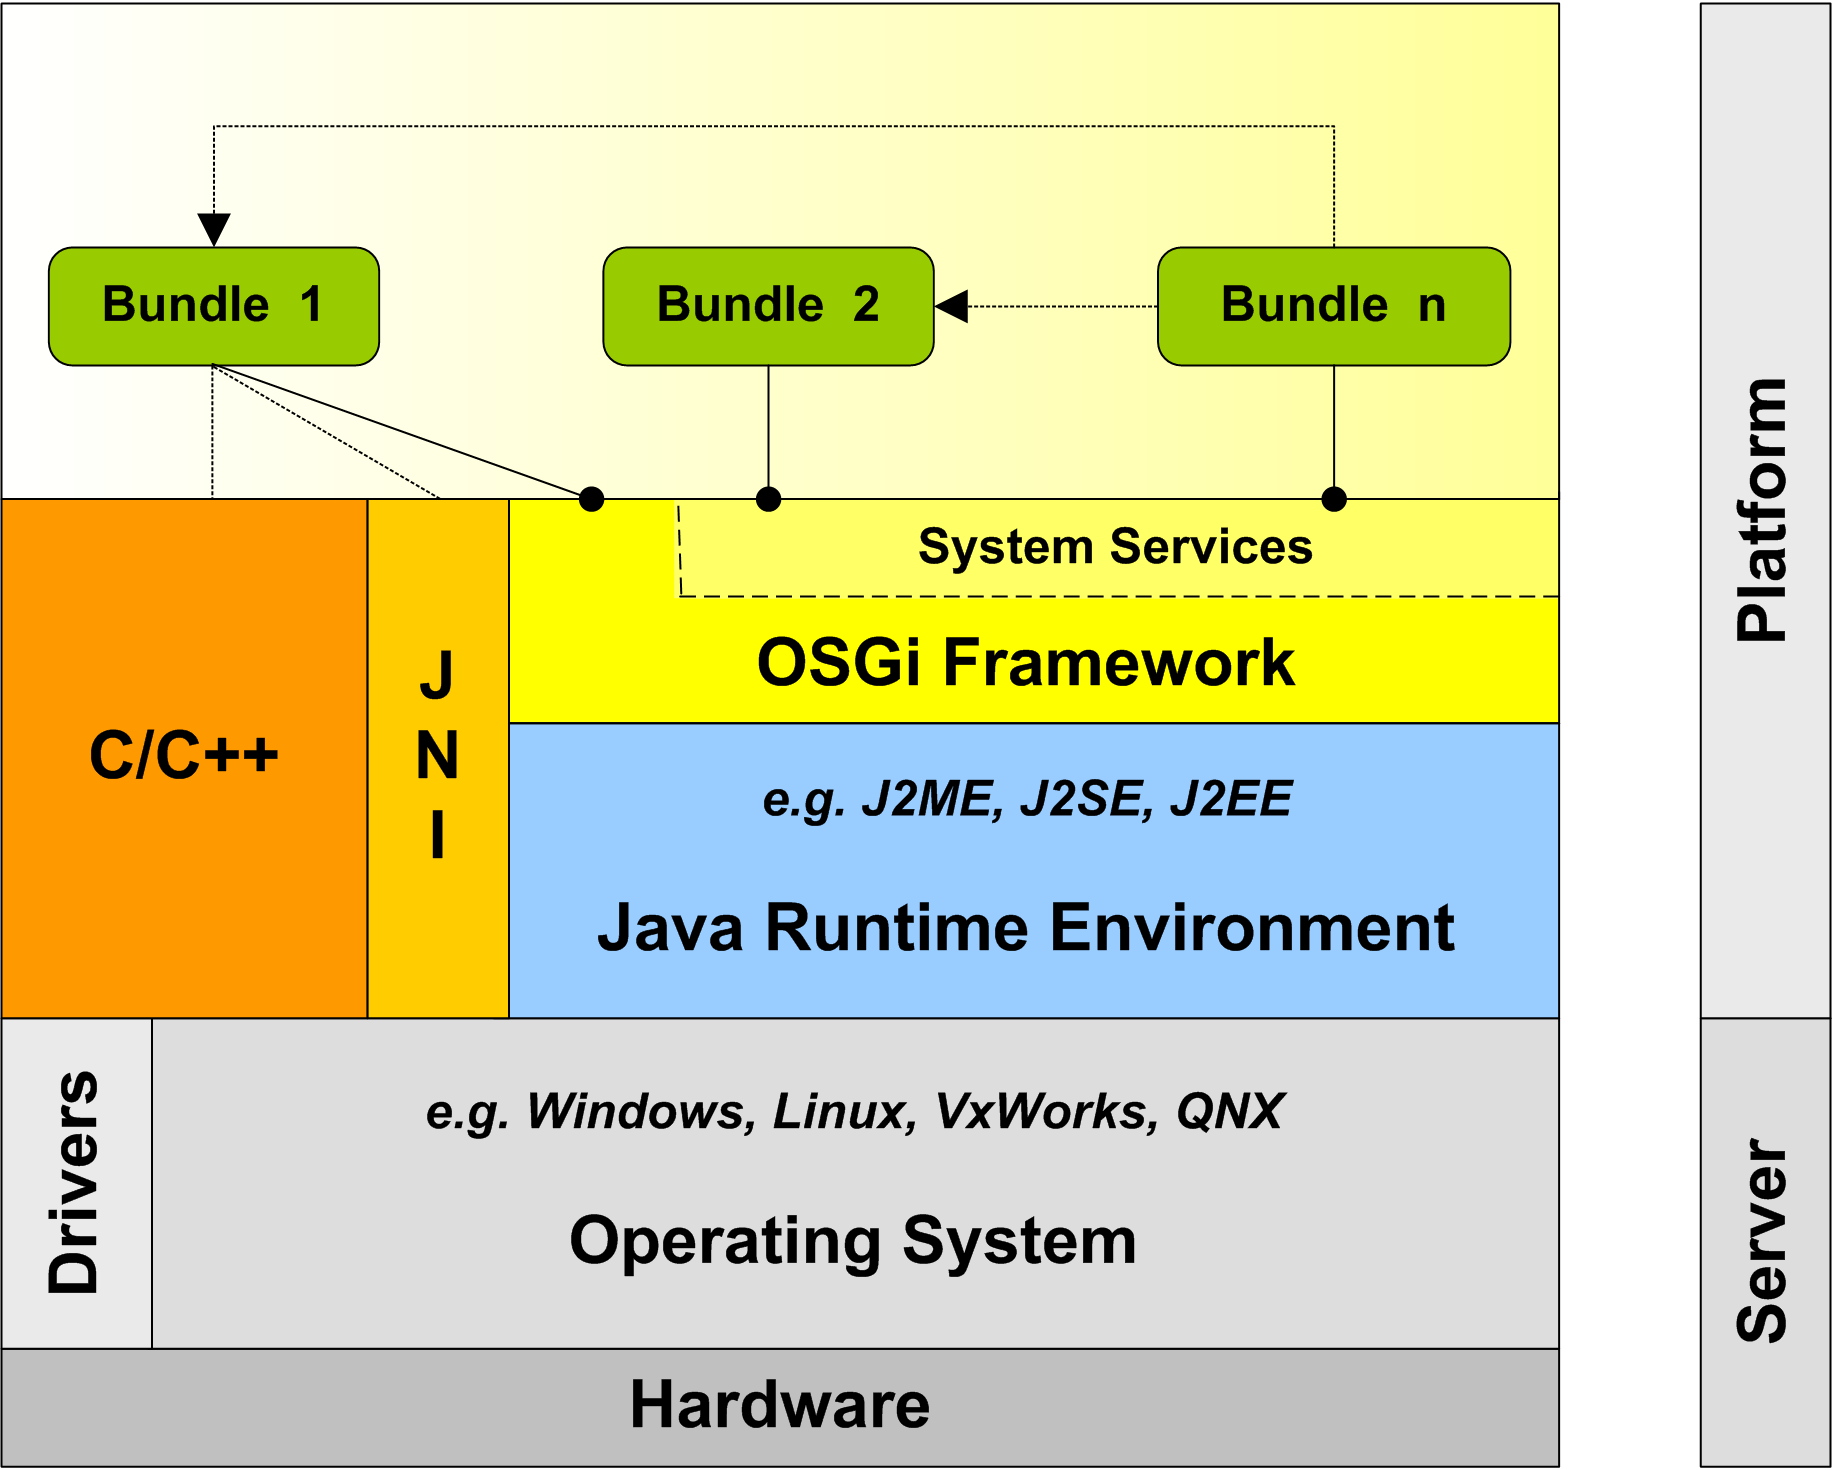
\includegraphics[scale=2]{pics/osgi_layer.png}
	\caption[OSGi layers]{
	\textbf{OSGi layers.}
	something}
	\end{center}
	\label{fig:osgi_layer}
\end{figure}

\subsection{Bundles}
Ein Bundle ist nach OSGi Spezifikation\citep{osgi_2009} eine technische Einheit
von Klassen und Ressourcen, die eigentständig in der Anwenung gestartet,
gestoppt, installiert und deinstalliert werden kann.
\index{Bundle}

Ressourcen und Klassen
eines Bundles können anderen Bundles bereitgestellt werden. Dazu müssen sie vom
bereitstellenden Bundle explizit exportiert werden und durch das nutzende
Bundle explizit importiert werden. Jedes Bundle stellt einen
Bundlenamen, der üblicherweise von der enthaltenen Paketstruktur
abgeleitet wird, sowie eine Versionsnummer bereit. Aus diesen beiden Komponenten
wird dann eine eindeutige Identifizierung des Bundles generiert.
So ist es beispielsweise möglich, ein und das selbe Bundle in unterschiedlichen
Versionierungen zu installieren.

Über die \first{MANIFEST.MF}, die ohnehin in jedem Jar-File vorhanden ist, wird
das Bundle neben dem Namen und der Version mit weiteren Meta-Informationen, wie
importierte und exportierte Pakete oder Lauzeitumgebung, ausgestattet.
\index{MANIFEST.MF}

Jedes Bundle ist innerhalb des Frameworks mit einem eigenen Class-Loader
ausgestattet, über welchen ausschliesslich die Bundle-eigenen Klassen geladen
werden. Auf diese Weise sind die einzelen Bundles strikt voneinander getrennt und die
Import-Export-Beziehungen zwischen den Bundles können explizit gesteuert
werden. 
Neben anderen Vorteilen, wie etwa das Installieren des selben Bundles in
unterschiedlichen Versionen, wird auf diese Weise das vollständig
dynamische Hinzufügen und Entfernen von Bundles erst ermöglicht, da der
Class Path des Class Loaders nach dessen Instanziierung nicht mehr verändert
werden kann.
\citep{wtherich_die_2008}
% selbe version 17
% importieren, exportieren 13,79
% class loading 89
% MANIFEST.MF 21
% lebenszyklen 23,55
% unterschied Bundle / Plug-In 41

\subsection{Services} % 93
Ein Service ist ein Java-Object, typischerweise ein Interface, das unter dem
Interface-Namen an der Service Registry angemeldet wird.
\index{Service Registry}
Die Service Registry steht bundleübergreifend in der Anwendung zu Verfügung.
Wird ein bestimmer Dienst von einem Bundle benötigt, kann dieser an der Service
Registry abgefragt werden, ohne dass im Enzelnen bekannt sein muss, welche
Implementierung dahinter steckt oder welches Bundle diesen Dienst anbietet.
\index{Bundle}
% Services können kommen und gehen 23
% Standard Services 13,25
\citep{wtherich_die_2008}
\section{Design}
\section{Genvorhersage}
